\begin{figure}[ht]
    \centering
    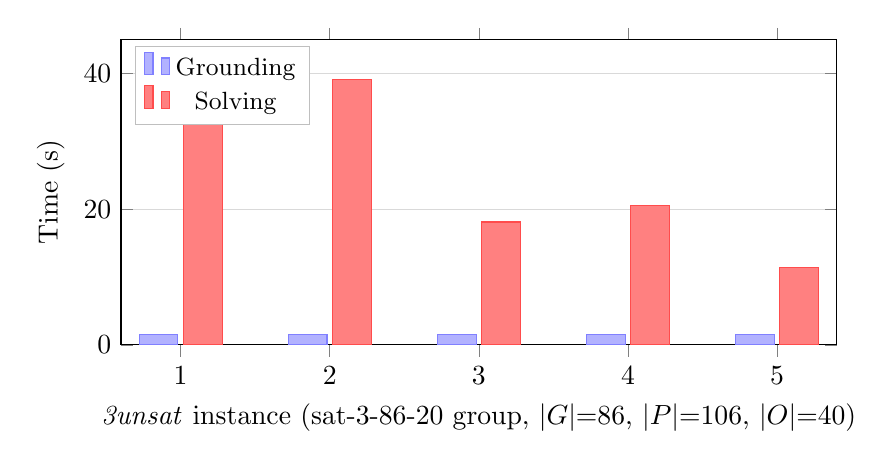
\begin{tikzpicture}
        \begin{axis}[
                ybar,
                width=0.88\textwidth,
                height=0.45\textwidth,
                ylabel={Time (s)},
                symbolic x coords={inst-1,inst-2,inst-3,inst-4,inst-5},
                xtick=data,
                xticklabels={1,2,3,4,5},
                xlabel={\textit{3unsat} instance (sat-3-86-20 group, $|G|{=}86$, $|P|{=}106$, $|O|{=}40$)},
                legend style={
                        font=\small,
                        at={(0.02,0.98)},
                        anchor=north west,
                        draw=gray!50,
                    },
                bar width=14pt,
                ymin=0, ymax=45,
                grid=major,
                grid style={gray!30},
                ymajorgrids=true,
                xmajorgrids=false,
            ]
            % Grounding (nearly constant)
            \addplot[fill=blue!30, draw=blue!50] coordinates {
                    (inst-1,1.4634) (inst-2,1.4804) (inst-3,1.481) (inst-4,1.4956) (inst-5,1.4674)
                };
            \addlegendentry{Grounding}
            % Solving (high variance)
            \addplot[fill=red!50, draw=red!70] coordinates {
                    (inst-1,33.51) (inst-2,39.19) (inst-3,18.12) (inst-4,20.54) (inst-5,11.36)
                };
            \addlegendentry{Solving}
        \end{axis}
    \end{tikzpicture}
    \caption{Grounding vs.\ solving time for five \textit{3unsat} instances with identical problem structure ($|G|{=}86$, $|P|{=}106$, $|O|{=}40$). Grounding time is constant (${\approx}\,1.48$s, ${\pm}\,2\%$); solving time varies by a factor of 3.5, reflecting instance-specific combinatorial difficulty.}
    \label{fig:3unsat_variance}
\end{figure}
